
\subsection{FL Research}\label{subsection:fl_research}

\begin{figure}[h]
    \centering
    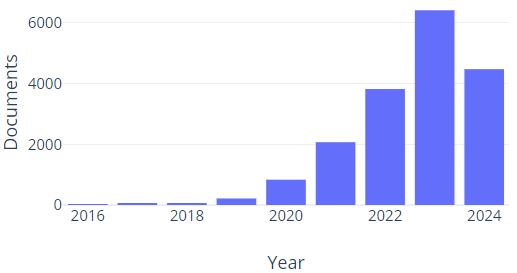
\includegraphics[width=0.8\textwidth]{fl_documents_research.png}
    \caption{Evolution of FL Publications}
    \label{fig:fl_documents_research}
\end{figure}

Figure \ref{fig:fl_documents_research} shows the exponential growth of FL documents since 2016.
(This data comes from searching for "federated learning" in article title, abstract, or keywords via Scopus \cite{scopus_homepage}.)
The idea for this graph is based on \cite{thesis:tum_fl_framework_comparison}.
Graph \ref{fig:fl_documents_research} uses a different query with the latest available data.

Before creating FLOps, we looked for research gaps in the fields of ML at the edge, specifically FL.
We have read and examined 47 papers in detail, with 26 papers focusing on FL. 
Additionally, we consulted several articles, joined and participated in discussion forums, and completed a couple of paid courses.
Discussing each paper in detail would heavily bloat this thesis.
This subsection presents key and meta-findings instead.
While working through the material, we created and incrementally updated a database in which we noted specific properties of each paper.
These properties include one or multiple categories in which the paper fits in.
Additional properties include the initial problems or challenges the authors tried to resolve, their contributions, results, limitations, and envisioned future work.
We also noted what ML or FL frameworks or libraries they claimed to use.

Table \ref{table:fl_research_table_1} depicts a subset of the analyzed FL papers.
It presents the documented contributions, limitations, and future work properties.
The remaining FL papers are available in Appendix \ref{appendix:fl_research}.
Note that we omit some of the 26 FL papers from these tables because we discuss them in greater detail throughout the background section.
These tables provide a good impression of the examined FL papers.
The following is a broad aggregated overview of a subset of these papers and their technical outcomes.
More precise individual insights of the examined paper are available in the mentioned tables.
Several papers \cite{paper:fl_inference_anytime_anywhere,paper:hfl_with_momentum_acceleration_in_multi_tier_networks,paper:model_pruning_for_edge_fl,paper:tackling_objective_inconsistency_problem_in_heterogeneous_fl} proposed novel learning methods that improve handling non-IID data, reduce resource usage, improve model quality, or train models quicker than previous methods.
Besides inventing or improving learning methods, others \cite{paper:refl_resource_efficient_fl,paper:edge_fl_via_mqtt_and_oma_lightweight_m2m,paper:fedat_high_performance_communication_efficient_fl_with_asynch_tiers} focus on new learner selection or aggregation algorithms to benefit the most from the available resources, especially from heterogeneous data.
Many works \cite{paper:edgefl_framework,paper:global_fl_platform_for_iot,paper:adaptive_exper_models_for_pfl} investigate the benefits and downsides of using different architectures for FL that lead to more efficient, performant, and scalable FL.
Other works \cite{paper:hfl_with_privacy, paper:cluster_based_secure_aggregation_for_fl,paper:efficient_privacy_preserving_ml_in_hierarchical_distributed_systems} focus on new privacy and security schemas or improve existing secure aggregation algorithms to reduce existing overheads and bottlenecks when using conventional protection.
A large portion of the examined works investigated and proved novel concepts to achieve a range of goals, from better privacy, scalability, and less overhead to better resource utilization.
Examples include \cite{paper:decentralized_edge_intelligence_dynamic_resource_allocation_framework_hfl,hpfl_over_massive_mobile_edge_computing_networks,paper:fl_toward_on_demand_client_deployment_at_edge}.
Patterns and trends can be extracted from these papers based on the documented properties.

\begin{figure}[p]
    \begin{changemargin}{-2cm}{0cm}
    \begin{tabular}{|c||m{0.4\paperwidth}|m{0.4\paperwidth}|}
        \hline
            ID & Contributions & Limitations \& Future Work \\
        \hline
            \cite{paper:refl_resource_efficient_fl}
            &
            A novel selection and staleness-aware aggregation strategy.
            Analysis of resource wastage and the impact of stragglers.
            A smart participation selection based on learner availability.
            &
            Privacy or security were not considered.
            Evaluations are based on classic datasets (MNIST, CIFAR-10), which do not reflect real non-IID data.
            Only homogeneous resources were assumed.
            Use of a simple linear regression model for availability prediction.
            More sophisticated alternatives exist.
            Factors such as battery level, bandwidth, and user preferences should also be considered for availability prediction.
        \\
        \hline
            \cite{paper:cluster_based_secure_aggregation_for_fl}
            &
            A novel cluster-based secure aggregation strategy for diverse nodes.
            Clustering based on processing score \& GPS information/latency leads to better throughput and reduces false-positive dropouts.
            A new additive sharing-based masking scheme that is robust against dropouts.
            &
            All participants are assumed to be honest.
            Malicious users were not considered.
            The aggregator might become a bottleneck, which can be resolved via HFL (with cluster heads).
            Image classification was the only evaluated ML task.
        \\
        \hline
            \cite{paper:privacy_preserving_deep_fl_for_coop_hierarchical_caching_in_fog_computing}
            &
            An FL caching scheme including novel algorithms and architecture.
            Utilization of an AI training model that considers user history.
            &
            A convergence analysis was not provided.
            For further security and privacy improvements, blockchain-empowered FL should be investigated.
        \\
        \hline
            \cite{paper:model_pretraining_and_initialization_for_fl}
            &
            Analysis of the impact of pre-training ML models for FL initialization compared to the common random approach.
            Findings show pre-trained model superiority.
            &
            It is challenging to get a pre-trained model if the necessary data is not available or private.
            Using pre-trained models can lead to biases.
            Only a specific (warm-start) initialization strategy was considered.
        \\
        \hline
            \cite{paper:decentralized_edge_intelligence_dynamic_resource_allocation_framework_hfl}
            &
            A novel incentive/resource-based allocation schema that utilizes game theory.
            Learners with more data are more valuable and they can compete for higher participation rewards.
            Multiple model owners compete for cluster heads with the most data.
            &
            The effects of social networks and their impact on worker's cluster selection decisions should be researched.
            Malicious workers were not considered.
        \\
        \hline
            \cite{paper:fedat_high_performance_communication_efficient_fl_with_asynch_tiers}
            &
            Synergy of asynchronous and synchronous FL via asynchronous tiers, which is able to handle stragglers.
            &
            The tiers all update the server individually.
            Further improvements are possible via HFL with intermediate cluster heads to do the aggregation.
            Additional security could be applied at these cluster heads.
        \\
        \hline
    \end{tabular}
    \captionof{table}{FL Papers considered for FLOps - Part I} 
    \label{table:fl_research_table_1}
\end{changemargin}

\end{figure}

\begin{figure}[p]
    \centering
    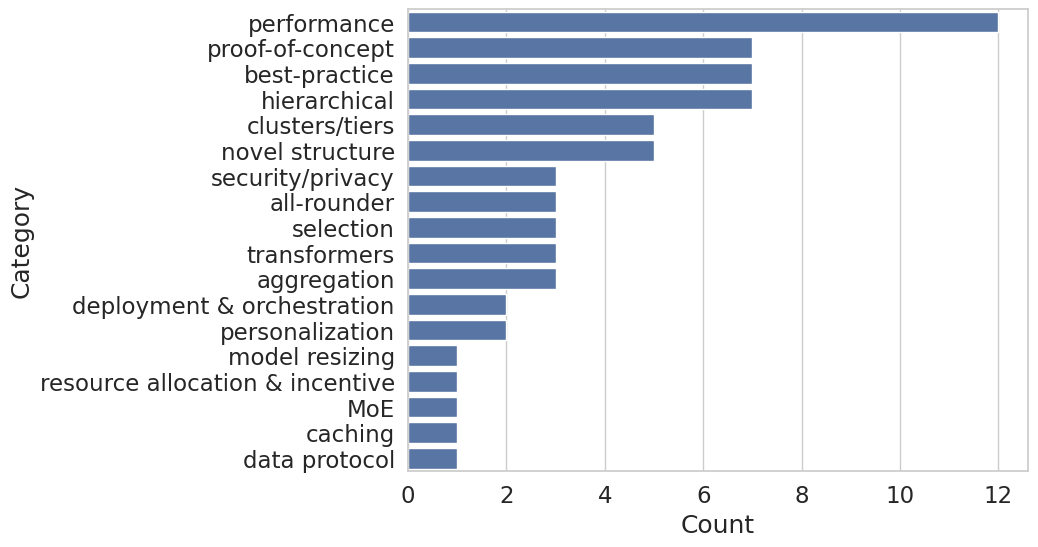
\includegraphics[width=1.0\textwidth]{fl_research_categories.png}
    \caption{FL Paper Categories}
    \label{fig:fl_research_categories}

    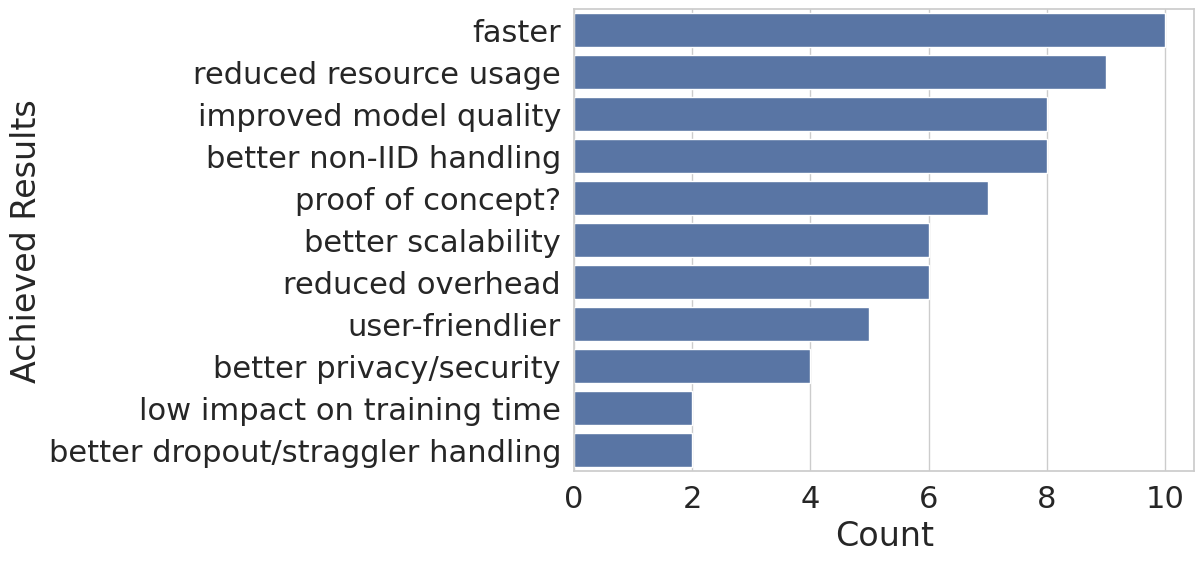
\includegraphics[width=0.9\textwidth]{fl_research_achieved_results.png}
    \caption{Achieved Results of FL Papers}
    \label{fig:fl_research_achieved_results}
\end{figure}

Patterns and trends help to better understand the research field of FL as a whole.
Figure \ref{fig:fl_research_categories} shows the different categories and their distribution.
Most examined papers focused on performance, trying new concepts, finding best practices, and exploring different FL architectures.
Only two papers focused on deployment and orchestration.

The achieved results match these categories.
Figure \ref{fig:fl_research_achieved_results} shows that these contributions lead to more efficient FL.
Improved aspects include speed, resource utilization, training results, and handling of heterogeneous data.
Additional insights about the research problems, contributions, limitations, and future work of the examined FL papers are available in the appendix \ref{appendix:fl_research}.

These documented properties might be biased, and the inspected sample size of papers is relatively small.
To improve confidence in these findings, we compare them with the total number of published works about FL.
Figure \ref{fig:fl_publications_compared} depicts how many works have been published in FL with specific keywords that match our custom categories.
We applied the same method to gather the data as for \ref{fig:fl_documents_research}.
The global results paint a similar picture as our samples.
The most popular topics in FL are related to privacy/security, performance, or algorithms.
Only a tiny portion of FL papers focus on usability, automation, orchestration, or other initial steps.

It seems that researchers assume others to already have working FL environments.
Furthermore, they seem to motivate their readers to optimize these setups based on their findings instead of replicating and configuring such an FL setup initially.
These tendencies are visible when inspecting the ML and FL frameworks and libraries the authors mentioned they used.
The following figure is again based on our examined papers.
Figure \ref{fig:fl_research_ml_and_fl_frameworks} shows that most authors did not explicitly state what ML framework or library they used for their work.
Many researchers used Pytorch and TensorFlow.
The figure also shows that FL researchers rarely mention what FL frameworks they use for their work.
It is much more common for authors to mention what ML framework they used than what FL framework they used.
Possible reasons for this might be that ML as a field is a lot older, more sophisticated, widespread, and established.
The same applies to ML frameworks.
On the other hand, FL is a very young subfield of ML research.
FL frameworks are still in their early stages.
FL researchers might be using FL frameworks.
However, due to the framework's immaturity, the researchers might not deem it important to explicitly point out that they used them.
Another possible explanation is that FL researchers are experts in FL and can set up and configure FL from the ground up.
Either way, this lack of transparency makes reproducing or extending their work challenging, if not infeasible.
These gaps in FL research motivated the creation of FLOps.

\begin{figure}[p]
    \centering
    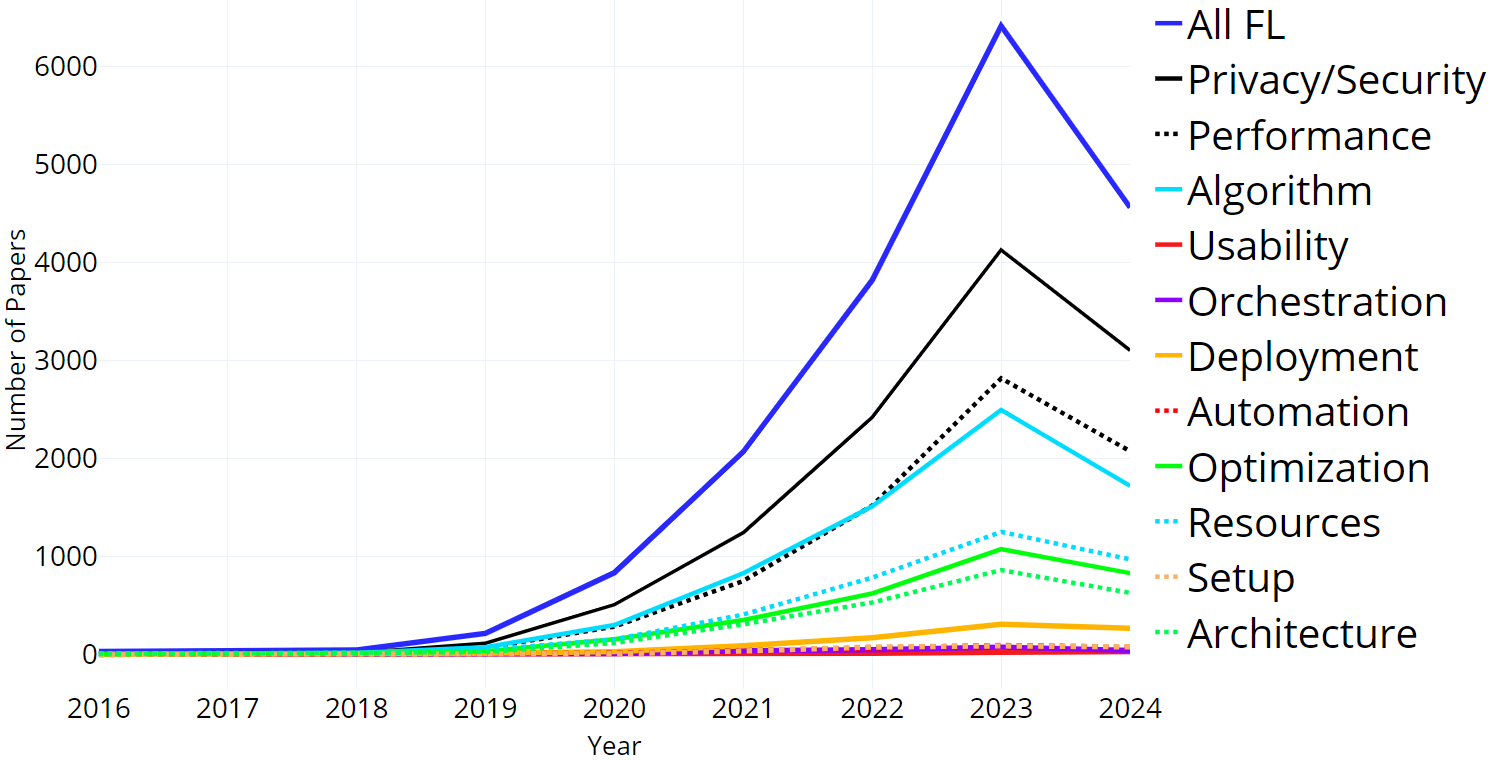
\includegraphics[width=1.0\textwidth]{fl_publications_compared.png}
    \caption{Evolution of FL Publications based on Keywords}
    \label{fig:fl_publications_compared}
    \vspace{2cm}
    \begin{adjustwidth}{-0.1\paperwidth}{-0.1\paperwidth}
        \centering
        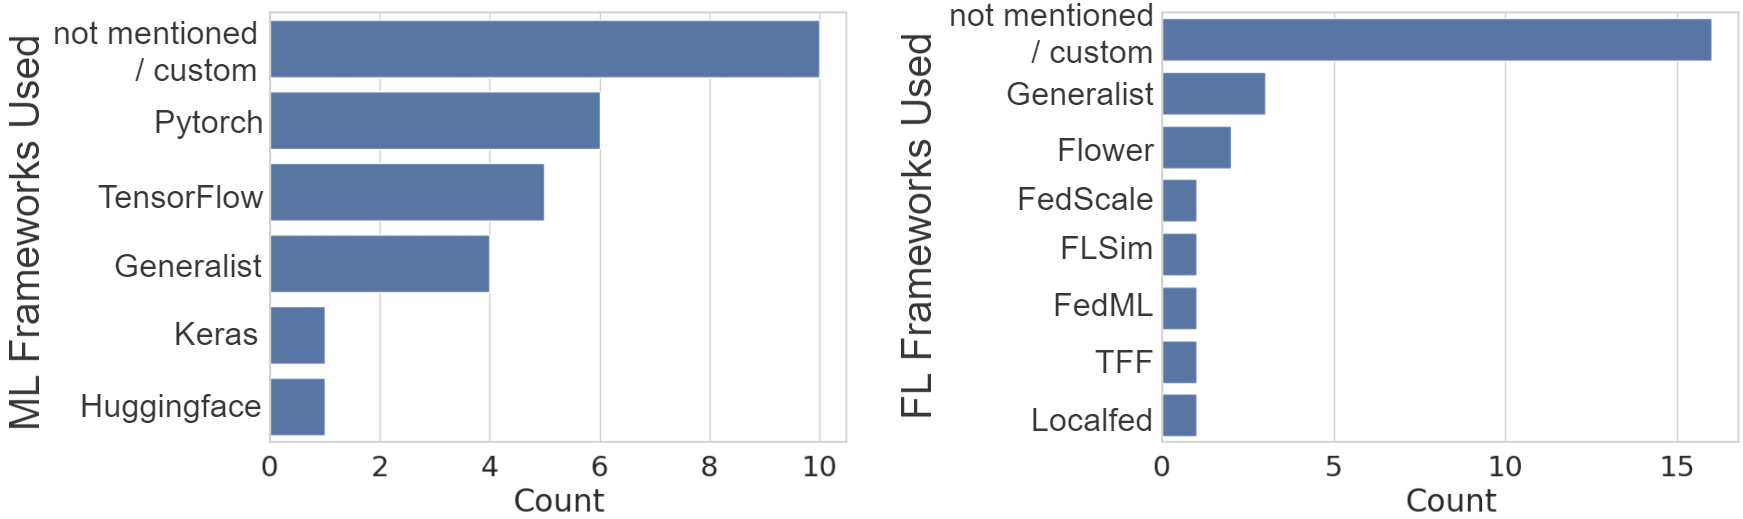
\includegraphics[width=0.8\paperwidth]{fl_research_ml_and_fl_frameworks.png}
        \caption{Distribution of mentioned ML and FL Frameworks in FL Papers}
        \label{fig:fl_research_ml_and_fl_frameworks}
    \end{adjustwidth}
\end{figure}

\pagebreak